\section{Mobile Web Development} % (fold)
\label{sec:mobile}

Web development has been, from the beginning, device independent.
Every device can access the same page and format it differently to a certain screen resolution.
Of course some of the less powerful devices suffered restrictions, since they could not handle \idx{JavaScript}, full \ida{CSS} or even images.

With the rise of touch devices like the \idx{iPhone} or the \idx{Android} phones, it appeared a new wave of mobile browsers capable of render websites almost as exactly as desktop browsers.
The beautiful thing about these new mobile browsers is that they are all based on the \idx{Webkit} engine.

\begin{figure}[htbp]
  \centering
    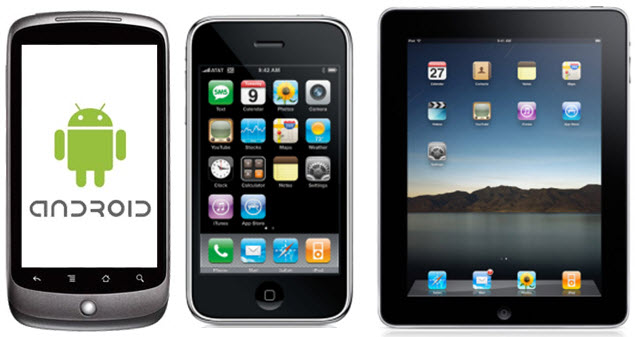
\includegraphics[width=\textwidth]{iphone-ipad-android}
  \caption[Mobile devices with Webkit]{An iPhone, iPad and Android, the three most popular mobile platforms that run Webkit}
  \label{fig:iphone-ipad-android}
\end{figure}

They can display more or less features, but they are somewhat homogenous in their implementation.
Also, since they are very recent, modern standards like \ida{HTML}5 and \ida{CSS}3 are widely supported.

The most important thing to notice is that the user input is notably different from a traditional computer.
Instead of using a mouse to go to an exact pixel in the screen, the user directly touches the display with his fingers.
This calls for new paradigms, since not all interfaces are cut for this kind of interaction:

\begin{itemize}
  \item Buttons must be bigger, since fingers are not as precise as mouses.
  \item The whole interface need to be at a certain size, since a good mobile web application should not require the user to zoom to see the content.
  This usually means less information in the screen.
  \item More than one finger can be used, in contrast to only one mouse in the desktop.
  That enables several new gestures, like pinching, that are newly available to web applications.
  \item By default, drag\et{}drop is reserved to scroll the page.
  If the web application needs to use it, like the current web interface does, it has to capture all finger events and re-create the scrolling experience.
  \item Double tapping is a movement that makes more sense on these devices than in desktop web applications, and it could be seen as a right click gesture on the desktop.
  \item There is also very important to notice that the screen could be oriented in portrait or landscape, so the interface must be adaptable.
\end{itemize}

The current \idx{ScaleNet} interface, being optimized for big screens, it is not even usable on these devices.
Even when zooming manually, most actions rely on drag\et{}drop and therefore are not even accessible, so it is impossible to move or delete a session.
It is clear that if these devices have to be supported, a mobile version needs to be developed fixing those issues.

To deal with these peculiarities, there are several additions to the web stack tools to make nicer web applications.
This applies specially in \idx{iOS} devices, but \idx{Android} also understands some of them.
The most useful and distinct features are:

\begin{description}
  \item[Touch events] Since mouse events do not make any sense there, special custom events for \emph{touches} and gestures are available.
  \item[Viewport] To deal with the fact that most websites are developed for bigger screens, by default web applications are rendered against a virtual viewport wider than the real screen.
  Then, it is up to the user to zoom in to read the page.
  
  At the same time, web applications specially designed for these devices can detect them and define the size of the viewport, so the user do not have to zoom to have a decent experience.
  Another solution is the use of \idx{CSS}3 conditional styles and media queries.
  \item[Special forms] While maintaining most of the form elements, there are some missing ---like file uploading--- and some new interface elements ---like select boxes.
  There are extra features that can be triggered like autocompletion, autocorrection, autocapitalize, custom keyboards for numbers/emails, etc.
  Moreover, since the virtual keyboard could appear, web applications should be prepared for having very little room.
  \item[App icon] Both \idx{iOS} and \idx{Android} allow the creation of shortcuts to display in the home screens.
  For that, it is possible to define the icons that those shortcuts can use.
  \item[Hiding the browser \ida{UI}] Once a web application is launched from an \idx{iOS} shortcut, it can dictate if the browser \ida{UI} should be hidden or not.
  In the case that the \ida{UI} is hidden, it can also define which aspect should the menubar have (light, dark or transparent).
  \item[Startup image] Native \idx{iOS} apps can specify a startup image to be displayed when loading the application.
  More than being a visual triviality, it is designed to display an empty interface so that the user \emph{feels} that the application loads faster.
  Web applications can also set such an image with a meta tag.
\end{description}

\begin{wrapfigure}{r}{0.5\textwidth}
  \centering
    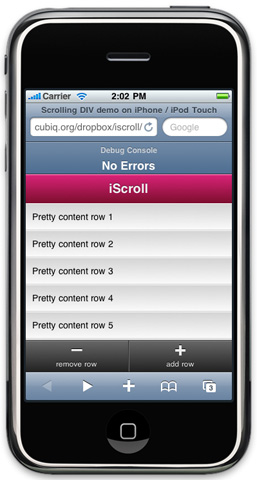
\includegraphics[width=0.48\textwidth]{iscroll}
  \caption{iScroll in action}
  \label{fig:iscroll}
\end{wrapfigure}

Lastly, it has to be noted that there are mobile \idx{JavaScript} frameworks that have been developed with these restrictions in mind.
Some of them try to bring a lightweight framework like \idx{Zepto.js}, others try to develop a full solution for web applications like \idx{Sencha} or \idx{JQTouch}, and others just try to ease the development of specific features.

For this project, one of those frameworks was used: \idx{iScroll}\footnote{\url{http://cubiq.org/iscroll}}.
The goal of this script is to provide a scrolling effect inside an element, since the only scrolling available in these mobile browsers is the page scrolling.
With mostly three lines of setup, this script simulates that native scrolling effect with some advanced \ida{CSS}3 properties (animations and so on).

The common use case for this effect is the implementation of a bottom toolbar, like in native apps.
These mobile browsers do not offer support for fixed positioned elements, so this is the only way that this kind of toolbar can be simulated.

% section mobile (end)